\section{Einleitung}
Seit Beginn der Menschheitsgeschichte gab es bereits unzählige Pandemien, welche ihren Tribut gefordert haben. Die neuste Pandemie, auch bekannt unter dem Namen \gls{covid19}, ist hierbei keine Ausnahme und zählt zu den Spitzenreitern in Bezug auf die tägliche Anzahl krankheitsbedingter Todesfälle nach einer Erkrankung (siehe Abbildung 1).

\begin{figure}[ht]
    \includegraphics[width=12cm]{images/krankheitsbedingte_todesfälle_nach_erkrankung.png}
    \centering
    \caption{Durchschnittliche tägliche Anzahl krankheitsbedingter Todesfälle weltweit nach Erkrankung (Stand:
1. Januar 2021) ~\citep[S. 12]{worldwide_epidemic_cases_study}}
\end{figure}

\gls{covid19}, fortlaufend als Corona bezeichnet, hat sowohl in den wirtschaftlichen als auch in den sozialen Strukturen tiefgreifende Veränderungen herbeigeführt. Um die Bevölkerung auf die Gefahr der Pandemie zu sensibilisieren und die rasant steigenden Fallzahlen (siehe Abbildung 2) des Virus einzudämmen, wurden diverse Anstrengungen unternommen.

\begin{figure}[ht]
    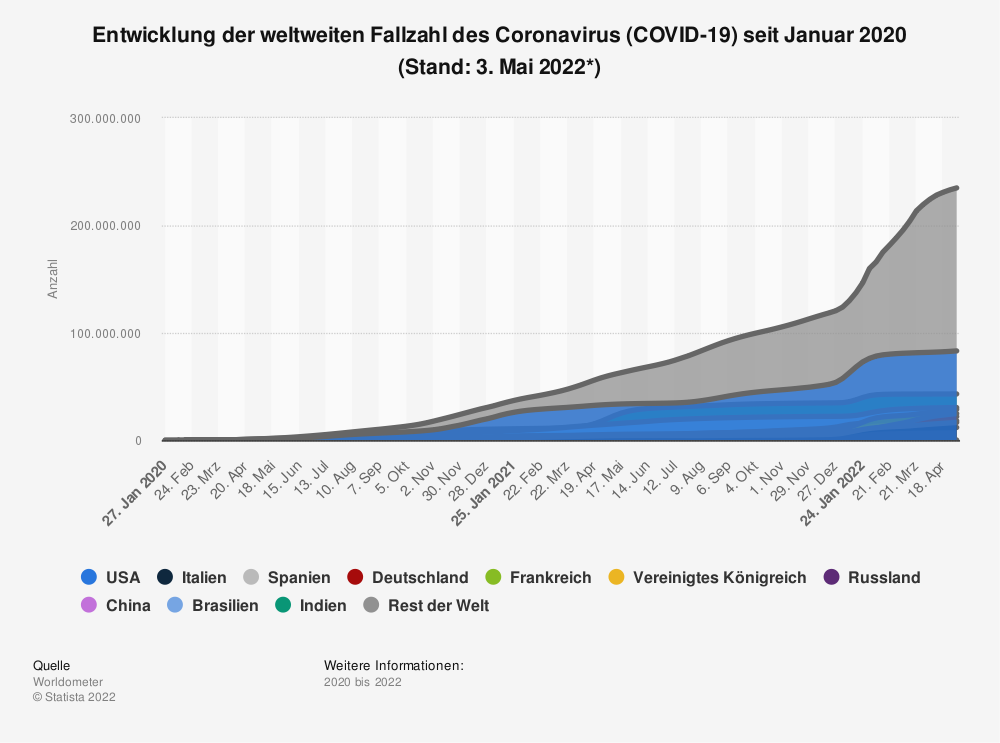
\includegraphics[width=10cm]{images/corona_fallzahlen.png}
    \centering
    \caption{Entwicklung der weltweiten Fallzahl des Coronavirus (COVID-19) seit Januar 2020 ~\citep{covid_cases_worldwide}}
\end{figure}

Eine zentrale Rolle spielten hierbei \textit{Datenvisualisierungen}. Wichtig in diesem Kontext zu verstehen ist, dass sich der Begriff Datenvisualisierungen nicht nur aus Linien- oder Kuchendiagrammen definiert, sondern ein breites Spektrum von verschiedenen Visualisierungen, darunter auch Infografiken, abdeckt. So erstellte zum Beispiel das \gls{bfs} diverse Infografiken in den Bereichen Gesundheit, Kultur sowie Kriminalität, in Bezug auf Corona ~\citep{covid19_bfs_infografiken}.

Besonders während einer weltweiten Pandemie wie Corona ist eine akkumulierte Sicht von verschiedenen Visualisierungsarten von zentraler Bedeutung. Dies kann mit Hilfe von \textit{Dashboards} bewerkstelligt werden. Der Begriff Dashboard kommt ursprünglich aus dem Englischen und bezieht sich auf das Armaturenbrett des Autos, wo alle relevanten Informationen übersichtlich auf einem Blick sichtbar sind ~\citep{term_definition_dashboard}. In Bezug auf Corona werden auf Dashboards unter anderem wichtige Informationen wie Ansteckungszahlen und Todesfälle visualisiert. Ein Beispiel für ein Dashboard ist das \textit{WHO Coronavirus Dashboard}, welches von der \gls{who} erstellt wurde ~\citep{who_dashboard}. Dass nebst dem in der Schweiz angesiedelten BFS selbst eine weltweite Organisation wie WHO sich um die Erstellung von Dashboards zur Corona Thematik bemüht, soll aufzeigen wie wichtig Datenvisualisierungen und insbesondere Dashboards geworden sind.

\subsection{Stand der Forschung}
 Die Coronavirus-Pandemie greift seit ihrem Aufkommen im Jahr 2019 in eine Vielzahl von Lebensbereichen ein. Es ist wenig verwunderlich, dass zu einem solch einschneidendem Thema eine grosse Anzahl von wissenschaftlichen Publikationen erstellt worden sind. Nachfolgend wird auf die wichtigsten bereits bestehenden Studien eingegangen, welche sich mit Corona Datenvisualisierungen sowie mit Dashboards im Allgemeinen beschäftigen.
 
 \subsubsection{Die Landschaft der Corona Datenvisualisierungen}
 Eine massgebende Studie um einen Überblick über die \textit{Landschaft der Corona Datenvisualisierungen} zu erhalten, ist die Studie von Zhang. Bei dieser Studie wurden rund 668 Corona Datenvisualisierungen im Zeitraum vom 22. Januar bis zum 31. Juli 2020 analysiert. Ein wichtiges Auswahlkriterium bei diesen Visualisierungen war, dass die allgemeine Bevölkerung als Zielgruppe im Fokus stand. Anschliessend wurden diese Visualisierungen sowohl mittels \textit{deduktiver} als auch \textit{induktiver} Codierung in Form eines Codebooks zusammengefasst ~\citep[S. 3]{yixuan_zhang}. Aus dem erstellten Codebook sind ebenfalls verschiedene \textit{Nachrichtenkategorien} sowie die dazugehörigen \textit{Visualisierungsarten} ersichtlich. Eine Nachrichtenkategorie beschreibt hierbei die Intention der Datenvisualisierungen (zum Beispiel Information über den Schweregrad der Pandemie). Unter die Kateogrie Visualisierungsarten fallen zum Beispiel Liniendiagramme etc. Beim Erstellen des Codebooks wurde zudem ein \textit{konzeptionelles Framework zum Verständnis von Datenvisualisierungen in Krisenzeiten} erstellt (siehe Abbildung 3). Die Studie von Zhang fokusierte sich hierbei primär auf die ersten drei Aspekte des Models (\textit{who uses what data to communicate what message in what form}). 
 
 \begin{figure}[ht]
    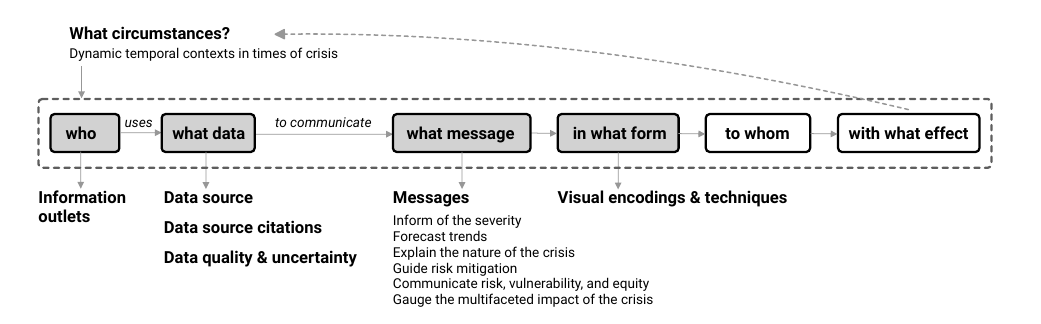
\includegraphics[width=12cm]{images/zhang_conceptual_framework.png}
    \centering
    \caption{Konzeptionelles Framework zum Verständnis von Datenvisualisierungen in Krisenzeiten ~\citep[S. 4]{yixuan_zhang}}
\end{figure}
 
\subsubsection{Corona-Dashboards}
Während der Corona Pandemie sind eine Vielzahl von Dashboards angefertigt worden. Eine interessante Studie in diesem Zusammenhang ist die Studie von Ivankovic ~\citep{ivankovic}. Diese Studie untersuchte im Speziellen \textit{webbasierte Dashboards}. Konkret wurden hierbei Aspekte wie Funktion (Purpose), Inhalt und Daten (What) sowie die eigentliche Visualisierung (how they communicate COVID-19 data) untersucht. Aus den insgesamt 158 untersuchten Dashboards wurden anschliessend die Gemeinsamkeiten evaluiert. Hieraus entstanden anschliessend 7 zentrale Merkmale von webbasierten Dashboards (siehe Abbildung 4). Diese Merkmale bildeten anschliessend die Grundlage, um die 158 untersuchten Dashboards zu bewerten.
\clearpage

 \begin{figure}[ht]
    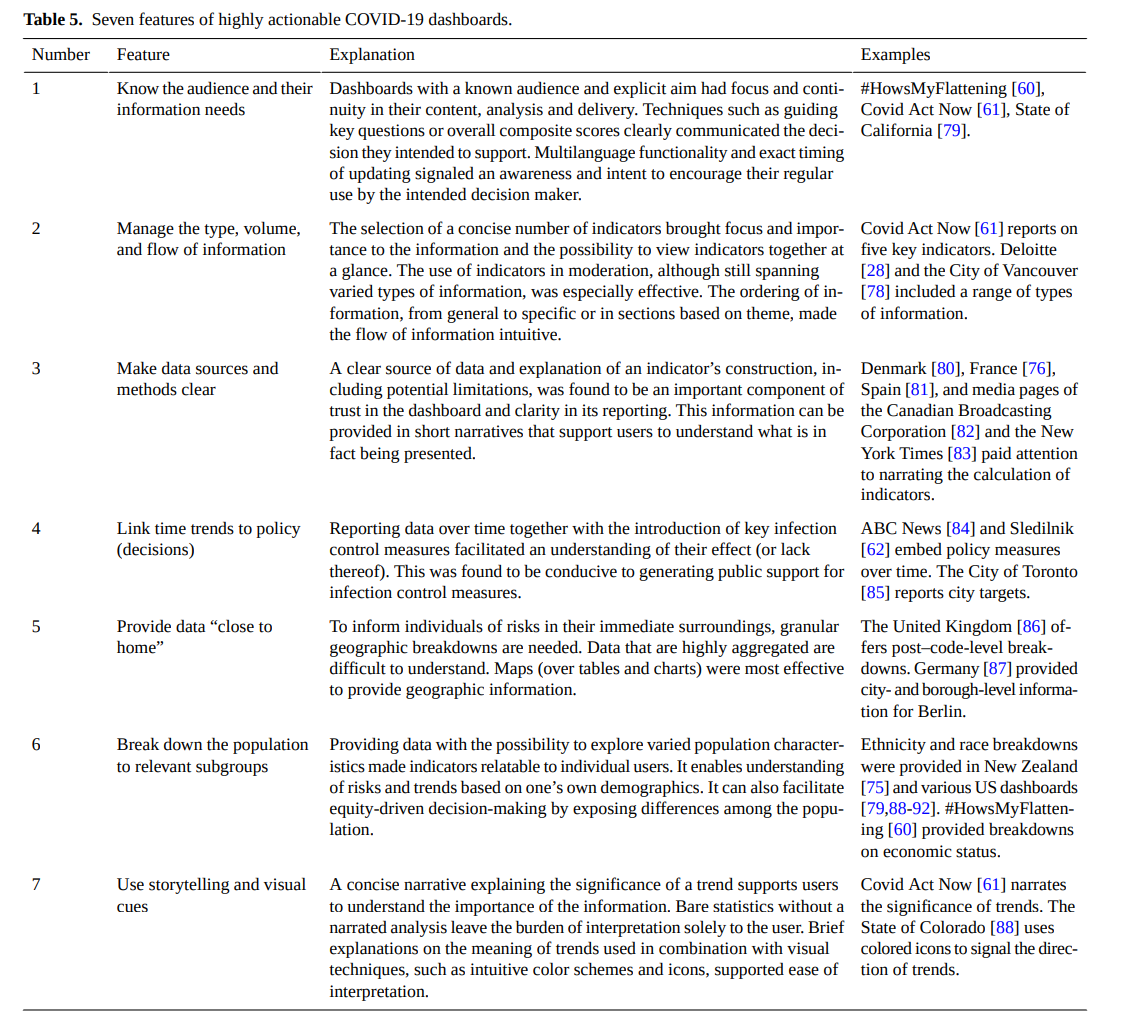
\includegraphics[width=10cm]{images/ivankovic_dashboard_characteristics.png}
    \centering
    \caption{Merkmale von webbasierten Dashboards gemäss Ivankovic ~\citep[S. 12]{ivankovic}}
\end{figure}


Es gibt aber auch Studien welche Corona-Dashboards aus dem Blickwinkel der Ersteller betrachten. Die Studie von Barbazza untersuchte die gesammelten Erfahrungen von rund 33 nationale Teams, welche für die Umsetzung von Corona-Dashboards verantwortlich waren. Die Studie geht hierbei konkret auf die gemachten Erfahrungen innerhalb der Teams im ersten Jahr der Pandemie ein. Hieraus wurden anschliessend allgemeine Barrieren (common barriers), Dinge welche unterstützend waren (enabler) sowie die gemachten Erfahrungen innerhalb der Teams (lessons) thematisiert ~\citep{barbazza}.

\subsection{Themenabgrenzung}
Die vorliegende Arbeit befasst sich mit Datenvisualisierungen, welche im Zuge der Corona-Pandemie erstellt worden sind. Jedoch wird der Hauptfokus der vorliegenden Arbeit gezielt auf \textbf{Corona-Dashboards} gelegt. Zum Einen erlauben Dashboards die \textit{Kombination} von verschiedenen Datenvisualisierungen, zum Anderen erlauben sie eine akummulierte Sicht auf die \textit{relevantesten Informationen} für eine bestimmte Zielgruppe. Die Wichtigkeit von Dashboards haben auch weltweite Regierungsorganisationen erkannt. Gemäss Barbazza war das \textit{webbasierte Dashboards} die bevorzugte Visualisierungsart von Regierungsorganisationen, wenn es darum geht, Informationen zur Corona-Pandemie darzustellen ~\citep{barbazza}.


\subsection{Zielsetzung und Forschungsfrage}
Die bestehenden Studien von Corona-Dashboards, sowie Datenvisualisierungen sprechen primär eine \textit{breite Zielgruppe} an. Zudem bieten bestehende Dashboards nach der Erstellung nur \textit{sehr begrenzte Anpassungsmöglichkeiten durch den Nutzer selbst}. Die vorliegende Arbeit möchte diese Lücke schliessen und formuliert daher folgende übergeordnete Fragestellung:

\begin{center}
\textbf{Wie stellen sich Millennials ein personalisierbares Corona Dashboard vor?}
\end{center}

Um diese Forschungsfrage abzudecken, wurden folgende untergeordnete Fragestellungen formuliert:

\begin{center}
\textbf{Welche Visualisierungsarten in Bezug auf Corona werden von Millennials gefordert?\\
(untergeordnete Forschungsfrage 1)}
\end{center}

\begin{center}
\textbf{Welche Informationen in Bezug auf Corona werden von Millennials gefordert?\\
(untergeordnete Forschungsfrage 2)}
\end{center}

\begin{center}
\textbf{Welche Personalisierungsmöglichkeiten werden von Millennials in Bezug auf Corona Dashboards gefordert?\\
(untergeordnete Forschungsfrage 3)}
\end{center}

\subsection{Methodische Vorgehensweise}
Da es sich bei der übergeordneten Forschungsfrage um eine Fragestellung mit explorativem Charakter handelt, wird für die Methodik das Design Science Research (\gls{dsr}) Modell nach Peffers verwendet (siehe Abbildung 5).


\begin{figure}[ht]
	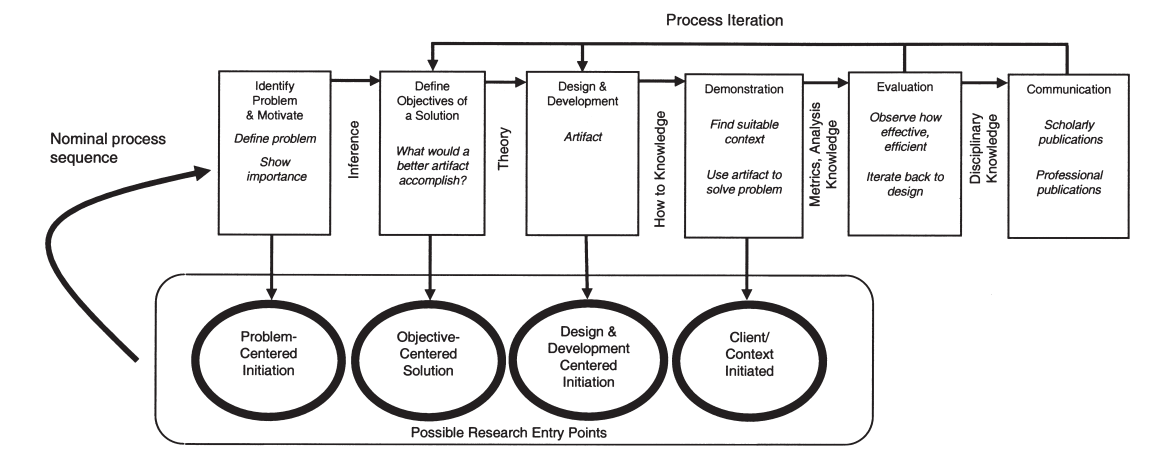
\includegraphics[width=12cm]{images/peffers_dsr_model.png}
	\centering
	\caption{DSR Modell nach Peffers ~\citep{peffers}}
\end{figure}

Bei diesem Modell gibt es mehrere Einstiegsmöglichkeiten (siehe \textit{Possible Research Entry Points}). Der Einstiegspunkt für die vorliegende Arbeit bildet der Punkt \textbf{Problem-Centered Initiation}. Das Problem, welches gelöst werden soll, ist die die starre Natur bestehender Corona Dashboards. Diese Dashboards lassen sich nach \textbf{der Erstellung für die angesprochene Zielgruppe} nur eingeschränkt anpassen oder personalisieren. In diesem Kontext ist die Entwicklung eines Prototyps interessant, welcher die Erstellung der Dashboards \textbf{in die Hände der Zielgruppe selbst legt} und so auch Personalisierungs- und Anpassungsmöglichkeiten bietet. Dies bildet somit die Grundlage für den ersten Schritt des Models \textit{Identify Problem und Motivation}. Im zweiten Schritt \textit{Define Objective of a Solution} geht es darum, das Ziel einer möglichen Lösung aufzuzeigen. Anschliessend geht es im Schritt \textit{Design und Development} um die eigentliche Erstellung des Artefakts, was im Zuge dieser Arbeit ein High Fidelity Prototyp darstellt. Anschliessend geht es in den nächsten Schritten noch um die Evaluation des erstellten Prototyps, sowie die Publikation der Ergebnisse. Jedoch beschränkt sich die vorliegende Arbeit auf die Erstellung eines Prototyps aufgrund teilstrukturierter Interviews mit Millennials. Die eigentliche Evaluation des Prototyps kann im Rahmen einer weiterführenden Arbeit evaluiert werden.

